%% Standalone figure: compile this file once (pdflatex debye_catastrophe.tex) to produce
%% debye_catastrophe.pdf, which main.tex includes with \includegraphics.
%% Recompile only after editing the figure.
%% Parameters are for water: p0 = 1.85 D, n = 3.34e22 cm^-3, eps_inf = 1.78.
\documentclass[11pt,tikz,border=2pt]{standalone}
\usepackage{amsmath,amssymb}       % \text, \vec, math symbols
\usepackage{pgfplots}              % Function plots with axes (log scale here)
\pgfplotsset{compat=1.18}
\usetikzlibrary{arrows.meta}       % Stealth arrow tips
\begin{document}
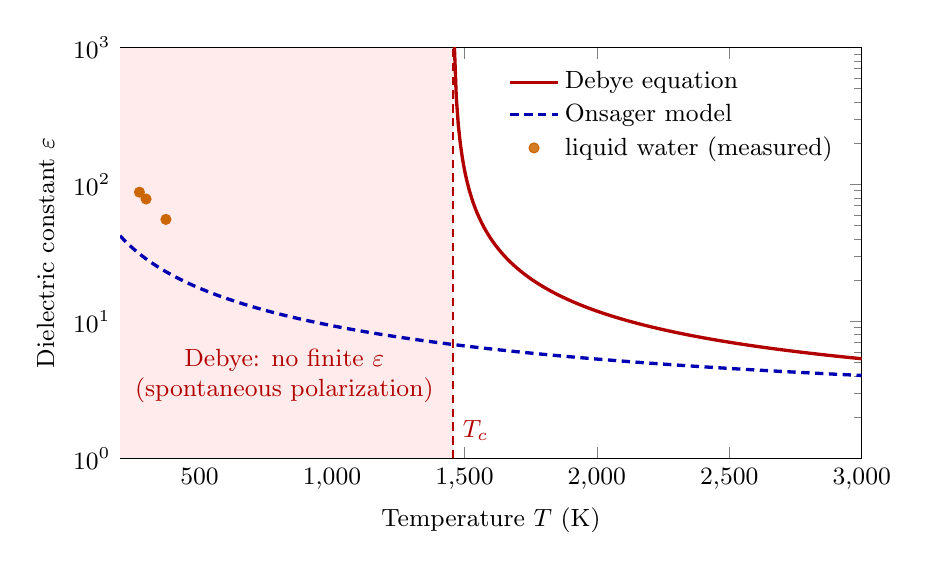
\begin{tikzpicture}[font=\small, >={Stealth[length=2mm]}]
  % Theta = 4 pi n p0^2 / (9 kB) in kelvin, eps_inf, and the Debye critical temperature
  \def\Th{1156}
  \def\einf{1.78}
  \def\Tc{1457}
  \begin{axis}[
      width=11cm, height=6.8cm,
      xmin=200, xmax=3000, ymin=1, ymax=1000,
      ymode=log,
      xlabel={Temperature $T$ (K)},
      ylabel={Dielectric constant $\varepsilon$},
      tick label style={font=\small},
      label style={font=\small},
      legend style={font=\small, draw=none, fill=white, fill opacity=0.85, text opacity=1,
                    at={(0.98,0.97)}, anchor=north east},
      legend cell align=left,
      clip=true,
    ]
    % region where the Debye equation has no finite positive solution
    \fill[red!8] (axis cs:200,1) rectangle (axis cs:\Tc,1000);
    \node[red!70!black, align=center, font=\small] at (axis cs:820,4)
      {Debye: no finite $\varepsilon$\\ (spontaneous polarization)};
    \draw[densely dashed, red!70!black] (axis cs:\Tc,1) -- (axis cs:\Tc,1000);
    \node[red!70!black, anchor=south west, font=\small] at (axis cs:\Tc,1.15) {$T_c$};

    % Debye equation: eps = (1 + 2y)/(1 - y), y = (eps_inf - 1)/(eps_inf + 2) + Theta/T
    \addplot[very thick, red!70!black, domain=1461.5:3000, samples=200]
      { (1 + 2*((\einf-1)/(\einf+2) + \Th/x)) / (1 - ((\einf-1)/(\einf+2) + \Th/x)) };
    \addlegendentry{Debye equation}

    % Onsager equation: 2 eps^2 - (eps_inf + K c) eps - eps_inf^2 = 0, K = Theta/T, c = (eps_inf+2)^2
    \addplot[very thick, blue!70!black, densely dashed, domain=200:3000, samples=200]
      { ((\einf + (\Th/x)*(\einf+2)^2) + sqrt((\einf + (\Th/x)*(\einf+2)^2)^2 + 8*\einf^2)) / 4 };
    \addlegendentry{Onsager model}

    % measured static dielectric constant of liquid water at 273 K, 298 K and 373 K
    \addplot[only marks, mark=*, mark size=1.8pt, orange!80!black]
      coordinates {(273,87.9) (298,78.4) (373,55.6)};
    \addlegendentry{liquid water (measured)}
  \end{axis}
\end{tikzpicture}
\end{document}
